\documentclass[10pt]{article}
\usepackage[margin=0.78in]{geometry}
\usepackage{amsmath,amssymb,booktabs,graphicx,hyperref,microtype}
\hypersetup{colorlinks=true,linkcolor=blue,urlcolor=blue}
\setlength{\parindent}{0pt}
\setlength{\parskip}{0.35em}
\newcommand{\PD}{\mathrm{PD}}
\newcommand{\PAX}{\mathrm{PAX}}

\title{A Data-Fitted Effective-Analyzer Model for\
\boldmath$\phi_2$-Dependent Output Amplitude in a Hybrid Mach--Zehnder Interferometer}
\author{Experiment analysis notes}
\date{13 August 2026}

\begin{document}
\maketitle

\begin{abstract}
This note derives and audits a data-fitted prediction of the $\phi_2$-dependent
power modulation measured at the two final outputs of a hybrid
Mach--Zehnder interferometer. A two-axis A-only/B-only/both-path calibration
fits an effective Stokes analyzer for each instrument. A later high-contrast
both-path fringe map supplies the current $\phi_1$ branch. The conditional
transfer calculation predicts mean $\phi_2$ fringe contrast $0.571$ at the
photodiode and $0.619$ in PAX \texttt{ptotal} units; the corresponding measured
means are $0.585$ and $0.657$. The contrast mean absolute errors are $0.027$
and $0.041$. This is evidence that the fitted model predicts modulation
\emph{magnitude}; it is not a blind prediction of fringe phase.
\end{abstract}

\section{Evidence and data sets}
The model coefficients came from
\texttt{192530\_field-model-calibration\_phi2-power-model-0/data.csv}.
That file contains $984$ simultaneous PAX/PD samples: four $\phi_1$ RP biases,
$41$ $\phi_2$ commands spanning the assumed $V_\lambda$, three blocking
conditions (path A only, path B only, and both paths), and forward/reverse
passes. Its SHA-256 prefix is \texttt{70aa7cfe62be8823}.

The transfer target is
\texttt{200934\_phi1-fringe-map\_phi1-fringe-map-1/data.csv}, containing
$714$ simultaneous PAX/PD samples with both paths open: $17$ $\phi_1$
commands, $21$ $\phi_2$ commands per fringe, and forward/reverse $\phi_1$
passes. Its SHA-256 prefix is \texttt{e8719481ab444339}.

The saved coefficient and comparison files are
\texttt{effective-analyzer-fit.csv} and
\texttt{phi2-amplitude-comparison.csv}; their SHA-256 prefixes are
\texttt{3c803a9e5ea4ecad} and \texttt{b59266a8c88eb988}, respectively.
These source files are retained in the experiment folders beside this paper.

\section{From ideal propagation to a detector-power model}
For the ideal equal-amplitude hybrid-MZI reference at the selected output port,
the PAX-convention Stokes vector is
\begin{equation}
\mathbf{S}(\alpha,\phi_2)=
\begin{bmatrix}
\cos\phi_2\\
\sin\phi_2\cos\alpha\\
\sin\phi_2\sin\alpha
\end{bmatrix},
\qquad \alpha=\phi_1+\delta\ \text{in the ideal static limit}.
\label{eq:stokes}
\end{equation}
The observed $\phi_1$ response is history dependent, so the analysis does not
force $\alpha$ to equal a linear RP-voltage scale. Instead, $\alpha$ is an
empirical branch coordinate.

The smallest model identifiable from the present two-axis data is a detector
response linear in Stokes state:
\begin{align}
P_d &= B_d+\mathbf{h}_d\cdot\mathbf{S}\\
&=B_d+h_{1,d}\cos\phi_2+
\left[h_{2,d}\cos\alpha+h_{3,d}\sin\alpha\right]\sin\phi_2.
\label{eq:analyzer}
\end{align}
Here $d\in\{\PD,\PAX\}$, while $B_d$ and $\mathbf{h}_d$ are in the native
units of that instrument. Equation~\eqref{eq:analyzer} is an \emph{effective}
analyzer model: it parameterizes the measured power response, but does not by
itself locate the particular nonideal optical component responsible.

At fixed $\alpha$, define
\begin{equation}
C_d=h_{1,d},\qquad
D_d=h_{2,d}\cos\alpha+h_{3,d}\sin\alpha.
\end{equation}
Then $P_d=B_d+C_d\cos\phi_2+D_d\sin\phi_2$, and the predicted amplitude and
contrast are
\begin{equation}
A_{d,\mathrm{pred}}=\sqrt{C_d^2+D_d^2},\qquad
\mathcal{C}_{d,\mathrm{pred}}=\frac{A_{d,\mathrm{pred}}}{B_d}.
\label{eq:contrast}
\end{equation}
The photodiode OD-2 attenuation changes its absolute voltage but cancels from
$\mathcal{C}$; PD volts and PAX \texttt{ptotal} units are never treated as an
absolute common power scale.

\section{Calibration coefficients}
For each detector and path condition, least squares fits the design row
\begin{equation}
\mathbf{x}=\left(1,\cos\phi_2,\sin\phi_2\cos\phi_1,
\sin\phi_2\sin\phi_1\right)
\end{equation}
to obtain $(B_d,h_{1,d},h_{2,d},h_{3,d})$. The both-path coefficients used in
the later transfer calculation are listed in Table~\ref{tab:coeff}.

\begin{table}[h]
\centering\small
\caption{Both-path effective-analyzer coefficients from the calibration.}
\label{tab:coeff}
\begin{tabular}{lrrrrrr}
\toprule
Detector & $B$ & $h_1$ & $h_2$ & $h_3$ & $R^2$ & RMS\\
\midrule
$\PD$ (V) & 0.2433345 & 0.1320399 & 0.0105049 & 0.0429494 & 0.900 & 0.03223\\
$\PAX$ (ptotal) & $2.311569\times10^{-4}$ & $-1.326148\times10^{-4}$ & $-9.59709\times10^{-6}$ & $-5.35634\times10^{-5}$ & 0.793 & $5.04244\times10^{-5}$\\
\bottomrule
\end{tabular}
\end{table}

The nonzero $\mathbf{h}_d$ values quantify the observed phase-to-power
dependence. In the ideal constant-total-power result, a true total-power
measurement would have no Stokes-dependent term.

\section{Measured fringe contrast and empirical branch selection}
At every fixed $\phi_1$ command and scan direction in the later map, each
detector is independently fit to
\begin{equation}
P_{d,\mathrm{meas}}=b_d+c_d\cos\phi_2+d_d\sin\phi_2.
\end{equation}
The measured contrast and phase are
\begin{equation}
\mathcal{C}_{d,\mathrm{meas}}=\frac{\sqrt{c_d^2+d_d^2}}{b_d},
\qquad \psi_d=\operatorname{atan2}(-d_d,c_d).
\label{eq:measured}
\end{equation}

The current phase branch is selected, independently at each $\phi_1$ command
and direction, by a dense numerical minimization over $\alpha\in[0,2\pi)$:
\begin{equation}
\alpha_* = \underset{\alpha}{\operatorname{argmin}}\ 
\sum_d\left[
\frac{h_{2,d}\cos\alpha+h_{3,d}\sin\alpha}{B_d}
-\frac{d_d}{b_d}\right]^2.
\label{eq:alpha}
\end{equation}
Equation~\eqref{eq:alpha} uses the later map's \emph{sine quadrature}, i.e.
fringe-phase information. It does \emph{not} use its measured contrast as an
input. Once $\alpha_*$ is selected, Eq.~\eqref{eq:contrast} produces the
predicted amplitude/contrast.

This distinction is essential: the result is a conditional transfer validation
of amplitude magnitude, not a blind future-state prediction of both phase and
amplitude.

\section{Worked calculation at forward $\phi_1=0$ RP V}
For this point, joint PD/PAX branch selection gives
$\alpha_*=0.032044\ \mathrm{rad}$. For the PD,
\begin{align}
\frac{C_{\PD}}{B_{\PD}}&=\frac{h_{1,\PD}}{B_{\PD}}=0.5426272,\\
\frac{D_{\PD}}{B_{\PD}}&=
\frac{h_{2,\PD}\cos\alpha_*+h_{3,\PD}\sin\alpha_*}{B_{\PD}}
=0.0488033,\\
\mathcal{C}_{\PD,\mathrm{pred}}&=
\sqrt{(C_{\PD}/B_{\PD})^2+(D_{\PD}/B_{\PD})^2}=0.5448174,\\
\mathcal{C}_{\PD,\mathrm{meas}}&=0.5457103.
\end{align}
For PAX, $(C/B,D/B)=(-0.5737002,-0.0489203)$, which gives
\begin{equation}
\mathcal{C}_{\PAX,\mathrm{pred}}=0.5757821,
\qquad \mathcal{C}_{\PAX,\mathrm{meas}}=0.5878357.
\end{equation}

\section{Aggregate comparison}
All $17$ $\phi_1$ commands and both directions are included ($N=34$ per
detector). Mean absolute error is defined by
\begin{equation}
\mathrm{MAE}_d=\frac{1}{N}\sum_{i=1}^{N}
\left|\mathcal{C}^{(i)}_{d,\mathrm{pred}}-
\mathcal{C}^{(i)}_{d,\mathrm{meas}}\right|.
\end{equation}

\begin{table}[h]
\centering\small
\caption{Predicted and measured $\phi_2$ fringe contrasts.}
\begin{tabular}{lrrrrrr}
\toprule
Detector & mean pred. & mean meas. & MAE & RMSE & bias & median relative error\\
\midrule
$\PD$ & 0.571 & 0.585 & 0.027 & 0.034 & $-0.014$ & 4.3\%\\
$\PAX$ & 0.619 & 0.657 & 0.041 & 0.048 & $-0.038$ & 6.1\%\\
\bottomrule
\end{tabular}
\end{table}

\begin{figure}[h]
\centering
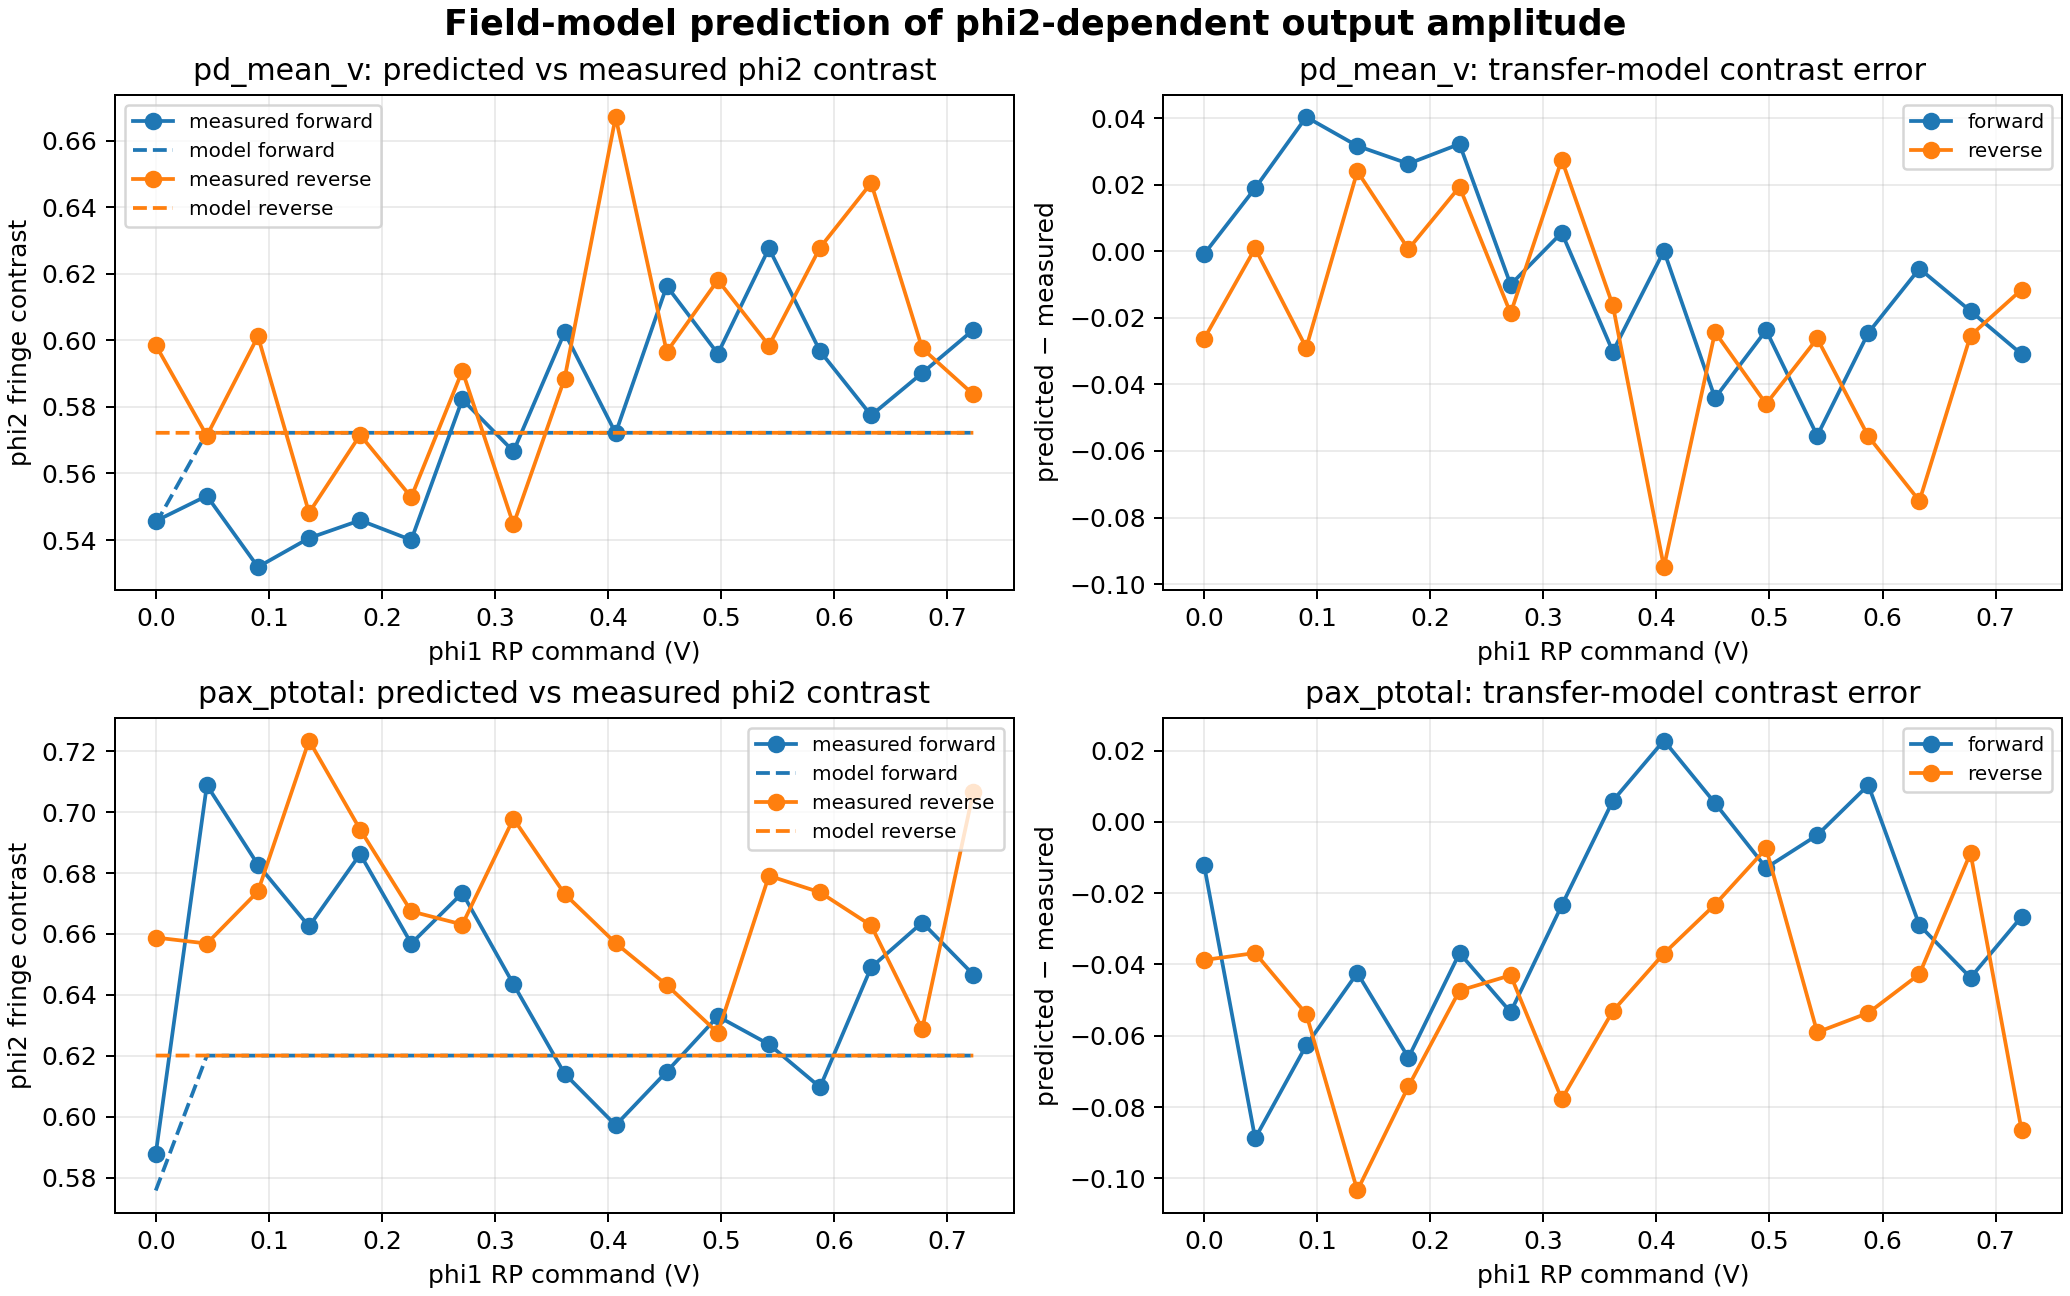
\includegraphics[width=0.97\linewidth]{phi2-amplitude-comparison.png}
\caption{Stored numerical comparison. Dashed traces are the conditional
effective-analyzer prediction; points are measured fringe contrasts.}
\end{figure}

\section{Interpretation and next experiment}
The calculation quantitatively captures the observed \emph{degree} of
$\phi_2$-dependent output modulation in both instruments. It therefore
supports a real, substantial phase-to-power term beyond the ideal
constant-power model. It does not uniquely distinguish nonideal beam splitting,
polarization leakage, mode overlap, path-dependent loss, or detector response;
multiple physical mechanisms can produce the same effective $\mathbf{h}_d$.

The most important limitation is that phase/quadrature transfer is not yet
clean and $\alpha$ was conditioned on the later map. The next decisive
experiment is a high-visibility \texttt{field-model-calibration} followed
immediately by \texttt{phi1-fringe-map}. Repeating the present calculation on
that state-matched pair will test whether the same model predicts amplitude
without the present run-to-run analyzer/branch mismatch.

\end{document}
